\documentclass[1p]{elsarticle_modified}
%\bibliographystyle{elsarticle-num}

%\usepackage[colorlinks]{hyperref}
%\usepackage{abbrmath_seonhwa} %\Abb, \Ascr, \Acal ,\Abf, \Afrak
\usepackage{amsfonts}
\usepackage{amssymb}
\usepackage{amsmath}
\usepackage{amsthm}
\usepackage{scalefnt}
\usepackage{amsbsy}
\usepackage{kotex}
\usepackage{caption}
\usepackage{subfig}
\usepackage{color}
\usepackage{graphicx}
\usepackage{xcolor} %% white, black, red, green, blue, cyan, magenta, yellow
\usepackage{float}
\usepackage{setspace}
\usepackage{hyperref}

\usepackage{tikz}
\usetikzlibrary{arrows}

\usepackage{multirow}
\usepackage{array} % fixed length table
\usepackage{hhline}

%%%%%%%%%%%%%%%%%%%%%
\makeatletter
\renewcommand*\env@matrix[1][\arraystretch]{%
	\edef\arraystretch{#1}%
	\hskip -\arraycolsep
	\let\@ifnextchar\new@ifnextchar
	\array{*\c@MaxMatrixCols c}}
\makeatother %https://tex.stackexchange.com/questions/14071/how-can-i-increase-the-line-spacing-in-a-matrix
%%%%%%%%%%%%%%%

\usepackage[normalem]{ulem}

\newcommand{\msout}[1]{\ifmmode\text{\sout{\ensuremath{#1}}}\else\sout{#1}\fi}
%SOURCE: \msout is \stkout macro in https://tex.stackexchange.com/questions/20609/strikeout-in-math-mode

\newcommand{\cancel}[1]{
	\ifmmode
	{\color{red}\msout{#1}}
	\else
	{\color{red}\sout{#1}}
	\fi
}

\newcommand{\add}[1]{
	{\color{blue}\uwave{#1}}
}

\newcommand{\replace}[2]{
	\ifmmode
	{\color{red}\msout{#1}}{\color{blue}\uwave{#2}}
	\else
	{\color{red}\sout{#1}}{\color{blue}\uwave{#2}}
	\fi
}

\newcommand{\Sol}{\mathcal{S}} %segment
\newcommand{\D}{D} %diagram
\newcommand{\A}{\mathcal{A}} %arc


%%%%%%%%%%%%%%%%%%%%%%%%%%%%%5 test

\def\sl{\operatorname{\textup{SL}}(2,\Cbb)}
\def\psl{\operatorname{\textup{PSL}}(2,\Cbb)}
\def\quan{\mkern 1mu \triangleright \mkern 1mu}

\theoremstyle{definition}
\newtheorem{thm}{Theorem}[section]
\newtheorem{prop}[thm]{Proposition}
\newtheorem{lem}[thm]{Lemma}
\newtheorem{ques}[thm]{Question}
\newtheorem{cor}[thm]{Corollary}
\newtheorem{defn}[thm]{Definition}
\newtheorem{exam}[thm]{Example}
\newtheorem{rmk}[thm]{Remark}
\newtheorem{alg}[thm]{Algorithm}

\newcommand{\I}{\sqrt{-1}}
\begin{document}

%\begin{frontmatter}
%
%\title{Boundary parabolic representations of knots up to 8 crossings}
%
%%% Group authors per affiliation:
%\author{Yunhi Cho} 
%\address{Department of Mathematics, University of Seoul, Seoul, Korea}
%\ead{yhcho@uos.ac.kr}
%
%
%\author{Seonhwa Kim} %\fnref{s_kim}}
%\address{Center for Geometry and Physics, Institute for Basic Science, Pohang, 37673, Korea}
%\ead{ryeona17@ibs.re.kr}
%
%\author{Hyuk Kim}
%\address{Department of Mathematical Sciences, Seoul National University, Seoul 08826, Korea}
%\ead{hyukkim@snu.ac.kr}
%
%\author{Seokbeom Yoon}
%\address{Department of Mathematical Sciences, Seoul National University, Seoul, 08826,  Korea}
%\ead{sbyoon15@snu.ac.kr}
%
%\begin{abstract}
%We find all boundary parabolic representation of knots up to 8 crossings.
%
%\end{abstract}
%\begin{keyword}
%    \MSC[2010] 57M25 
%\end{keyword}
%
%\end{frontmatter}

%\linenumbers
%\tableofcontents
%
\newcommand\colored[1]{\textcolor{white}{\rule[-0.35ex]{0.8em}{1.4ex}}\kern-0.8em\color{red} #1}%
%\newcommand\colored[1]{\textcolor{white}{ #1}\kern-2.17ex	\textcolor{white}{ #1}\kern-1.81ex	\textcolor{white}{ #1}\kern-2.15ex\color{red}#1	}

{\Large $\underline{12a_{1048}~(K12a_{1048})}$}

\setlength{\tabcolsep}{10pt}
\renewcommand{\arraystretch}{1.6}
\vspace{1cm}\begin{tabular}{m{100pt}>{\centering\arraybackslash}m{274pt}}
\multirow{5}{120pt}{
	\centering
	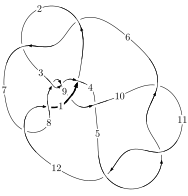
\includegraphics[width=112pt]{../../../GIT/diagram.site/Diagrams/png/1849_12a_1048.png}\\
\ \ \ A knot diagram\footnotemark}&
\allowdisplaybreaks
\textbf{Linearized knot diagam} \\
\cline{2-2}
 &
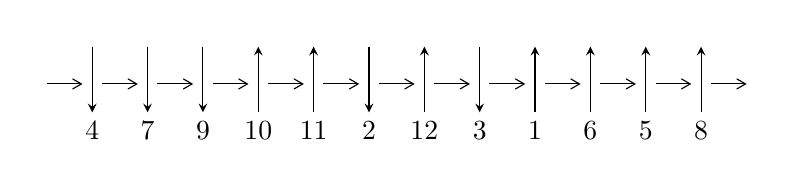
\begin{tikzpicture}[x=20pt, y=17pt]
	% nodes
	\node (C0) at (0, 0) {};
	\node (C1) at (1, 0) {};
	\node (C1U) at (1, +1) {};
	\node (C1D) at (1, -1) {4};

	\node (C2) at (2, 0) {};
	\node (C2U) at (2, +1) {};
	\node (C2D) at (2, -1) {7};

	\node (C3) at (3, 0) {};
	\node (C3U) at (3, +1) {};
	\node (C3D) at (3, -1) {9};

	\node (C4) at (4, 0) {};
	\node (C4U) at (4, +1) {};
	\node (C4D) at (4, -1) {10};

	\node (C5) at (5, 0) {};
	\node (C5U) at (5, +1) {};
	\node (C5D) at (5, -1) {11};

	\node (C6) at (6, 0) {};
	\node (C6U) at (6, +1) {};
	\node (C6D) at (6, -1) {2};

	\node (C7) at (7, 0) {};
	\node (C7U) at (7, +1) {};
	\node (C7D) at (7, -1) {12};

	\node (C8) at (8, 0) {};
	\node (C8U) at (8, +1) {};
	\node (C8D) at (8, -1) {3};

	\node (C9) at (9, 0) {};
	\node (C9U) at (9, +1) {};
	\node (C9D) at (9, -1) {1};

	\node (C10) at (10, 0) {};
	\node (C10U) at (10, +1) {};
	\node (C10D) at (10, -1) {6};

	\node (C11) at (11, 0) {};
	\node (C11U) at (11, +1) {};
	\node (C11D) at (11, -1) {5};

	\node (C12) at (12, 0) {};
	\node (C12U) at (12, +1) {};
	\node (C12D) at (12, -1) {8};
	\node (C13) at (13, 0) {};

	% arrows
	\draw[->,>={angle 60}]
	(C0) edge (C1) (C1) edge (C2) (C2) edge (C3) (C3) edge (C4) (C4) edge (C5) (C5) edge (C6) (C6) edge (C7) (C7) edge (C8) (C8) edge (C9) (C9) edge (C10) (C10) edge (C11) (C11) edge (C12) (C12) edge (C13) ;	\draw[->,>=stealth]
	(C1U) edge (C1D) (C2U) edge (C2D) (C3U) edge (C3D) (C4D) edge (C4U) (C5D) edge (C5U) (C6U) edge (C6D) (C7D) edge (C7U) (C8U) edge (C8D) (C9D) edge (C9U) (C10D) edge (C10U) (C11D) edge (C11U) (C12D) edge (C12U) ;
	\end{tikzpicture} \\
\hhline{~~} \\& 
\textbf{Solving Sequence} \\ \cline{2-2} 
 &
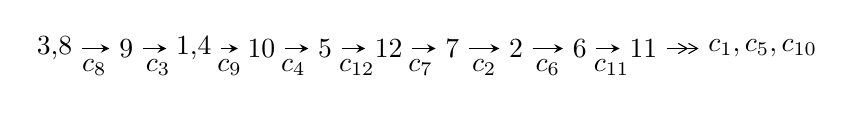
\begin{tikzpicture}[x=23pt, y=7pt]
	% node
	\node (A0) at (-1/8, 0) {3,8};
	\node (A1) at (1, 0) {9};
	\node (A2) at (33/16, 0) {1,4};
	\node (A3) at (25/8, 0) {10};
	\node (A4) at (33/8, 0) {5};
	\node (A5) at (41/8, 0) {12};
	\node (A6) at (49/8, 0) {7};
	\node (A7) at (57/8, 0) {2};
	\node (A8) at (65/8, 0) {6};
	\node (A9) at (73/8, 0) {11};
	\node (C1) at (1/2, -1) {$c_{8}$};
	\node (C2) at (3/2, -1) {$c_{3}$};
	\node (C3) at (21/8, -1) {$c_{9}$};
	\node (C4) at (29/8, -1) {$c_{4}$};
	\node (C5) at (37/8, -1) {$c_{12}$};
	\node (C6) at (45/8, -1) {$c_{7}$};
	\node (C7) at (53/8, -1) {$c_{2}$};
	\node (C8) at (61/8, -1) {$c_{6}$};
	\node (C9) at (69/8, -1) {$c_{11}$};
	\node (A10) at (11, 0) {$c_{1},c_{5},c_{10}$};

	% edge
	\draw[->,>=stealth]	
	(A0) edge (A1) (A1) edge (A2) (A2) edge (A3) (A3) edge (A4) (A4) edge (A5) (A5) edge (A6) (A6) edge (A7) (A7) edge (A8) (A8) edge (A9) ;
	\draw[->>,>={angle 60}]	
	(A9) edge (A10);
\end{tikzpicture} \\ 

\end{tabular} \\

\footnotetext{
The image of knot diagram is generated by the software ``\textbf{Draw programme}" developed by Andrew Bartholomew(\url{http://www.layer8.co.uk/maths/draw/index.htm\#Running-draw}), where we modified some parts for our purpose(\url{https://github.com/CATsTAILs/LinksPainter}).
}\phantom \\ \newline 
\centering \textbf{Ideals for irreducible components\footnotemark of $X_{\text{par}}$} 
 
\begin{align*}
I^u_{1}&=\langle 
1.21895\times10^{483} u^{122}-2.00271\times10^{482} u^{121}+\cdots+2.90201\times10^{482} b+1.95148\times10^{485},\\
\phantom{I^u_{1}}&\phantom{= \langle  }1.85948\times10^{485} u^{122}-3.93751\times10^{484} u^{121}+\cdots+3.97576\times10^{484} a+3.12400\times10^{487},\\
\phantom{I^u_{1}}&\phantom{= \langle  }u^{123}- u^{122}+\cdots+853 u-137\rangle \\
I^u_{2}&=\langle 
3615086 u^{24}+4785247 u^{23}+\cdots+2401109 b-9094340,\\
\phantom{I^u_{2}}&\phantom{= \langle  }-5355406 u^{24}+999159 u^{23}+\cdots+7203327 a+12279998,\;u^{25}-12 u^{23}+\cdots+4 u+3\rangle \\
\\
\end{align*}
\raggedright * 2 irreducible components of $\dim_{\mathbb{C}}=0$, with total 148 representations.\\
\footnotetext{All coefficients of polynomials are rational numbers. But the coefficients are sometimes approximated in decimal forms when there is not enough margin.}
\newpage
\renewcommand{\arraystretch}{1}
\centering \section*{I. $I^u_{1}= \langle 1.22\times10^{483} u^{122}-2.00\times10^{482} u^{121}+\cdots+2.90\times10^{482} b+1.95\times10^{485},\;1.86\times10^{485} u^{122}-3.94\times10^{484} u^{121}+\cdots+3.98\times10^{484} a+3.12\times10^{487},\;u^{123}- u^{122}+\cdots+853 u-137 \rangle$}
\flushleft \textbf{(i) Arc colorings}\\
\begin{tabular}{m{7pt} m{180pt} m{7pt} m{180pt} }
\flushright $a_{3}=$&$\begin{pmatrix}0\\u\end{pmatrix}$ \\
\flushright $a_{8}=$&$\begin{pmatrix}1\\0\end{pmatrix}$ \\
\flushright $a_{9}=$&$\begin{pmatrix}1\\u^2\end{pmatrix}$ \\
\flushright $a_{1}=$&$\begin{pmatrix}-4.67704 u^{122}+0.990379 u^{121}+\cdots+3876.46 u-785.763\\-4.20035 u^{122}+0.690110 u^{121}+\cdots+3393.47 u-672.456\end{pmatrix}$ \\
\flushright $a_{4}=$&$\begin{pmatrix}- u\\- u^3+u\end{pmatrix}$ \\
\flushright $a_{10}=$&$\begin{pmatrix}-1.36566 u^{122}-0.0177930 u^{121}+\cdots+1101.44 u-210.574\\-3.17578 u^{122}+0.515977 u^{121}+\cdots+2687.38 u-534.214\end{pmatrix}$ \\
\flushright $a_{5}=$&$\begin{pmatrix}1.79496 u^{122}-0.0577026 u^{121}+\cdots-1325.63 u+255.267\\4.80962 u^{122}-0.664266 u^{121}+\cdots-3857.94 u+760.602\end{pmatrix}$ \\
\flushright $a_{12}=$&$\begin{pmatrix}-0.476686 u^{122}+0.300269 u^{121}+\cdots+482.987 u-113.307\\-4.20035 u^{122}+0.690110 u^{121}+\cdots+3393.47 u-672.456\end{pmatrix}$ \\
\flushright $a_{7}=$&$\begin{pmatrix}-2.03889 u^{122}+0.462183 u^{121}+\cdots+1852.80 u-372.392\\8.25817 u^{122}-1.01878 u^{121}+\cdots-6665.60 u+1310.00\end{pmatrix}$ \\
\flushright $a_{2}=$&$\begin{pmatrix}-0.676402 u^{122}+0.255561 u^{121}+\cdots+610.368 u-132.811\\-5.46240 u^{122}+0.914876 u^{121}+\cdots+4421.91 u-877.990\end{pmatrix}$ \\
\flushright $a_{6}=$&$\begin{pmatrix}-2.63084 u^{122}+0.421127 u^{121}+\cdots+2131.33 u-416.137\\6.62526 u^{122}-0.866746 u^{121}+\cdots-5402.46 u+1065.21\end{pmatrix}$ \\
\flushright $a_{11}=$&$\begin{pmatrix}-4.44348 u^{122}+0.332202 u^{121}+\cdots+3545.17 u-687.481\\7.02325 u^{122}-0.491528 u^{121}+\cdots-5313.14 u+1030.01\end{pmatrix}$\\&\end{tabular}
\flushleft \textbf{(ii) Obstruction class $= -1$}\\~\\
\flushleft \textbf{(iii) Cusp Shapes $= -24.7292 u^{122}+2.72629 u^{121}+\cdots+19167.5 u-3758.32$}\\~\\
\newpage\renewcommand{\arraystretch}{1}
\flushleft \textbf{(iv) u-Polynomials at the component}\newline \\
\begin{tabular}{m{50pt}|m{274pt}}
Crossings & \hspace{64pt}u-Polynomials at each crossing \\
\hline $$\begin{aligned}c_{1}\end{aligned}$$&$\begin{aligned}
&u^{123}-4 u^{122}+\cdots+608612 u-35287
\end{aligned}$\\
\hline $$\begin{aligned}c_{2},c_{6}\end{aligned}$$&$\begin{aligned}
&u^{123}-2 u^{122}+\cdots+7280 u-1709
\end{aligned}$\\
\hline $$\begin{aligned}c_{3},c_{8}\end{aligned}$$&$\begin{aligned}
&u^{123}+u^{122}+\cdots+853 u+137
\end{aligned}$\\
\hline $$\begin{aligned}c_{4}\end{aligned}$$&$\begin{aligned}
&u^{123}- u^{122}+\cdots+310818 u+82413
\end{aligned}$\\
\hline $$\begin{aligned}c_{5},c_{10},c_{11}\end{aligned}$$&$\begin{aligned}
&u^{123}+u^{122}+\cdots+48 u+9
\end{aligned}$\\
\hline $$\begin{aligned}c_{7},c_{12}\end{aligned}$$&$\begin{aligned}
&u^{123}+2 u^{122}+\cdots+4 u+1
\end{aligned}$\\
\hline $$\begin{aligned}c_{9}\end{aligned}$$&$\begin{aligned}
&u^{123}-2 u^{122}+\cdots+2 u-1
\end{aligned}$\\
\hline
\end{tabular}\\~\\
\newpage\renewcommand{\arraystretch}{1}
\flushleft \textbf{(v) Riley Polynomials at the component}\newline \\
\begin{tabular}{m{50pt}|m{274pt}}
Crossings & \hspace{64pt}Riley Polynomials at each crossing \\
\hline $$\begin{aligned}c_{1}\end{aligned}$$&$\begin{aligned}
&y^{123}-24 y^{122}+\cdots+48933975036 y-1245172369
\end{aligned}$\\
\hline $$\begin{aligned}c_{2},c_{6}\end{aligned}$$&$\begin{aligned}
&y^{123}-84 y^{122}+\cdots+29345840 y-2920681
\end{aligned}$\\
\hline $$\begin{aligned}c_{3},c_{8}\end{aligned}$$&$\begin{aligned}
&y^{123}-87 y^{122}+\cdots+642943 y-18769
\end{aligned}$\\
\hline $$\begin{aligned}c_{4}\end{aligned}$$&$\begin{aligned}
&y^{123}-31 y^{122}+\cdots+104568100794 y-6791902569
\end{aligned}$\\
\hline $$\begin{aligned}c_{5},c_{10},c_{11}\end{aligned}$$&$\begin{aligned}
&y^{123}+109 y^{122}+\cdots+3186 y-81
\end{aligned}$\\
\hline $$\begin{aligned}c_{7},c_{12}\end{aligned}$$&$\begin{aligned}
&y^{123}-72 y^{122}+\cdots+112 y-1
\end{aligned}$\\
\hline $$\begin{aligned}c_{9}\end{aligned}$$&$\begin{aligned}
&y^{123}-8 y^{122}+\cdots+122 y-1
\end{aligned}$\\
\hline
\end{tabular}\\~\\
\newpage\flushleft \textbf{(vi) Complex Volumes and Cusp Shapes}
$$\begin{array}{c|c|c}  
\text{Solutions to }I^u_{1}& \I (\text{vol} + \sqrt{-1}CS) & \text{Cusp shape}\\
 \hline 
\begin{aligned}
u &= \phantom{-}0.943927 + 0.361878 I \\
a &= \phantom{-}0.908606 - 0.984560 I \\
b &= \phantom{-}1.316770 - 0.232966 I\end{aligned}
 & -1.14555 + 2.82046 I & \phantom{-0.000000 } 0 \\ \hline\begin{aligned}
u &= \phantom{-}0.943927 - 0.361878 I \\
a &= \phantom{-}0.908606 + 0.984560 I \\
b &= \phantom{-}1.316770 + 0.232966 I\end{aligned}
 & -1.14555 - 2.82046 I & \phantom{-0.000000 } 0 \\ \hline\begin{aligned}
u &= \phantom{-}0.875727 + 0.452631 I \\
a &= -0.01544 + 1.88890 I \\
b &= -1.13845 + 0.95496 I\end{aligned}
 & \phantom{-}1.15757 - 5.43534 I & \phantom{-0.000000 } 0 \\ \hline\begin{aligned}
u &= \phantom{-}0.875727 - 0.452631 I \\
a &= -0.01544 - 1.88890 I \\
b &= -1.13845 - 0.95496 I\end{aligned}
 & \phantom{-}1.15757 + 5.43534 I & \phantom{-0.000000 } 0 \\ \hline\begin{aligned}
u &= -0.891895 + 0.507585 I \\
a &= -0.01788 + 1.92967 I \\
b &= \phantom{-}1.10603 + 1.03544 I\end{aligned}
 & -3.38927 + 8.71767 I & \phantom{-0.000000 } 0 \\ \hline\begin{aligned}
u &= -0.891895 - 0.507585 I \\
a &= -0.01788 - 1.92967 I \\
b &= \phantom{-}1.10603 - 1.03544 I\end{aligned}
 & -3.38927 - 8.71767 I & \phantom{-0.000000 } 0 \\ \hline\begin{aligned}
u &= \phantom{-}1.026550 + 0.121549 I \\
a &= \phantom{-}0.386221 + 1.319250 I \\
b &= -1.198580 + 0.420234 I\end{aligned}
 & -2.46420 - 1.83999 I & \phantom{-0.000000 } 0 \\ \hline\begin{aligned}
u &= \phantom{-}1.026550 - 0.121549 I \\
a &= \phantom{-}0.386221 - 1.319250 I \\
b &= -1.198580 - 0.420234 I\end{aligned}
 & -2.46420 + 1.83999 I & \phantom{-0.000000 } 0 \\ \hline\begin{aligned}
u &= -0.157699 + 0.938275 I \\
a &= \phantom{-}0.277855 + 0.268995 I \\
b &= -1.232660 + 0.014196 I\end{aligned}
 & \phantom{-}3.44114 + 1.62193 I & \phantom{-0.000000 } 0 \\ \hline\begin{aligned}
u &= -0.157699 - 0.938275 I \\
a &= \phantom{-}0.277855 - 0.268995 I \\
b &= -1.232660 - 0.014196 I\end{aligned}
 & \phantom{-}3.44114 - 1.62193 I & \phantom{-0.000000 } 0\\
 \hline 
 \end{array}$$\newpage$$\begin{array}{c|c|c}  
\text{Solutions to }I^u_{1}& \I (\text{vol} + \sqrt{-1}CS) & \text{Cusp shape}\\
 \hline 
\begin{aligned}
u &= -1.014780 + 0.274190 I \\
a &= -0.94328 - 1.10444 I \\
b &= -1.269650 - 0.444108 I\end{aligned}
 & \phantom{-}2.74556 + 0.92758 I & \phantom{-0.000000 } 0 \\ \hline\begin{aligned}
u &= -1.014780 - 0.274190 I \\
a &= -0.94328 + 1.10444 I \\
b &= -1.269650 + 0.444108 I\end{aligned}
 & \phantom{-}2.74556 - 0.92758 I & \phantom{-0.000000 } 0 \\ \hline\begin{aligned}
u &= -1.061450 + 0.078503 I \\
a &= -0.88476 + 1.21857 I \\
b &= \phantom{-}1.099060 + 0.307206 I\end{aligned}
 & -8.31481 - 0.54476 I & \phantom{-0.000000 } 0 \\ \hline\begin{aligned}
u &= -1.061450 - 0.078503 I \\
a &= -0.88476 - 1.21857 I \\
b &= \phantom{-}1.099060 - 0.307206 I\end{aligned}
 & -8.31481 + 0.54476 I & \phantom{-0.000000 } 0 \\ \hline\begin{aligned}
u &= -1.053660 + 0.166811 I \\
a &= -0.82483 + 1.39823 I \\
b &= -0.402376 + 0.640368 I\end{aligned}
 & -6.90473 - 0.66791 I & \phantom{-0.000000 } 0 \\ \hline\begin{aligned}
u &= -1.053660 - 0.166811 I \\
a &= -0.82483 - 1.39823 I \\
b &= -0.402376 - 0.640368 I\end{aligned}
 & -6.90473 + 0.66791 I & \phantom{-0.000000 } 0 \\ \hline\begin{aligned}
u &= -0.708309 + 0.587971 I \\
a &= -0.825937 - 0.455610 I \\
b &= -1.347660 + 0.339095 I\end{aligned}
 & -1.94726 + 1.61762 I & \phantom{-0.000000 } 0 \\ \hline\begin{aligned}
u &= -0.708309 - 0.587971 I \\
a &= -0.825937 + 0.455610 I \\
b &= -1.347660 - 0.339095 I\end{aligned}
 & -1.94726 - 1.61762 I & \phantom{-0.000000 } 0 \\ \hline\begin{aligned}
u &= \phantom{-}1.074590 + 0.221218 I \\
a &= \phantom{-}1.00913 - 1.20136 I \\
b &= \phantom{-}1.27968 - 0.65261 I\end{aligned}
 & -1.19981 - 4.88070 I & \phantom{-0.000000 } 0 \\ \hline\begin{aligned}
u &= \phantom{-}1.074590 - 0.221218 I \\
a &= \phantom{-}1.00913 + 1.20136 I \\
b &= \phantom{-}1.27968 + 0.65261 I\end{aligned}
 & -1.19981 + 4.88070 I & \phantom{-0.000000 } 0\\
 \hline 
 \end{array}$$\newpage$$\begin{array}{c|c|c}  
\text{Solutions to }I^u_{1}& \I (\text{vol} + \sqrt{-1}CS) & \text{Cusp shape}\\
 \hline 
\begin{aligned}
u &= -1.084660 + 0.181582 I \\
a &= -0.31392 + 1.77188 I \\
b &= \phantom{-}1.091840 + 0.530231 I\end{aligned}
 & -2.13487 + 5.15770 I & \phantom{-0.000000 } 0 \\ \hline\begin{aligned}
u &= -1.084660 - 0.181582 I \\
a &= -0.31392 - 1.77188 I \\
b &= \phantom{-}1.091840 - 0.530231 I\end{aligned}
 & -2.13487 - 5.15770 I & \phantom{-0.000000 } 0 \\ \hline\begin{aligned}
u &= -0.900205\phantom{ +0.000000I} \\
a &= \phantom{-}1.02288\phantom{ +0.000000I} \\
b &= \phantom{-}1.98444\phantom{ +0.000000I}\end{aligned}
 & \phantom{-}4.01544\phantom{ +0.000000I} & \phantom{-0.000000 } 0 \\ \hline\begin{aligned}
u &= \phantom{-}0.895791 + 0.019019 I \\
a &= -1.009130 + 0.439876 I \\
b &= -1.95945 + 0.25495 I\end{aligned}
 & \phantom{-}0.12052 - 4.25089 I & \phantom{-0.000000 } 0 \\ \hline\begin{aligned}
u &= \phantom{-}0.895791 - 0.019019 I \\
a &= -1.009130 - 0.439876 I \\
b &= -1.95945 - 0.25495 I\end{aligned}
 & \phantom{-}0.12052 + 4.25089 I & \phantom{-0.000000 } 0 \\ \hline\begin{aligned}
u &= -0.820333 + 0.360106 I \\
a &= \phantom{-}0.10899 + 1.87087 I \\
b &= \phantom{-}1.23039 + 0.88663 I\end{aligned}
 & -2.13523 + 2.35342 I & \phantom{-0.000000 } 0 \\ \hline\begin{aligned}
u &= -0.820333 - 0.360106 I \\
a &= \phantom{-}0.10899 - 1.87087 I \\
b &= \phantom{-}1.23039 - 0.88663 I\end{aligned}
 & -2.13523 - 2.35342 I & \phantom{-0.000000 } 0 \\ \hline\begin{aligned}
u &= -0.595834 + 0.666999 I \\
a &= -0.752220 - 0.136772 I \\
b &= -1.254400 + 0.593067 I\end{aligned}
 & -2.54598 - 4.14695 I & \phantom{-0.000000 } 0 \\ \hline\begin{aligned}
u &= -0.595834 - 0.666999 I \\
a &= -0.752220 + 0.136772 I \\
b &= -1.254400 - 0.593067 I\end{aligned}
 & -2.54598 + 4.14695 I & \phantom{-0.000000 } 0 \\ \hline\begin{aligned}
u &= \phantom{-}0.628567 + 0.612338 I \\
a &= \phantom{-}0.721244 - 0.291562 I \\
b &= \phantom{-}1.253860 + 0.465398 I\end{aligned}
 & \phantom{-}1.83812 + 1.17430 I & \phantom{-0.000000 } 0\\
 \hline 
 \end{array}$$\newpage$$\begin{array}{c|c|c}  
\text{Solutions to }I^u_{1}& \I (\text{vol} + \sqrt{-1}CS) & \text{Cusp shape}\\
 \hline 
\begin{aligned}
u &= \phantom{-}0.628567 - 0.612338 I \\
a &= \phantom{-}0.721244 + 0.291562 I \\
b &= \phantom{-}1.253860 - 0.465398 I\end{aligned}
 & \phantom{-}1.83812 - 1.17430 I & \phantom{-0.000000 } 0 \\ \hline\begin{aligned}
u &= \phantom{-}1.011850 + 0.506765 I \\
a &= \phantom{-}0.20701 + 1.86271 I \\
b &= -0.803841 + 1.002100 I\end{aligned}
 & -4.71491 - 2.53383 I & \phantom{-0.000000 } 0 \\ \hline\begin{aligned}
u &= \phantom{-}1.011850 - 0.506765 I \\
a &= \phantom{-}0.20701 - 1.86271 I \\
b &= -0.803841 - 1.002100 I\end{aligned}
 & -4.71491 + 2.53383 I & \phantom{-0.000000 } 0 \\ \hline\begin{aligned}
u &= \phantom{-}1.124820 + 0.150846 I \\
a &= \phantom{-}0.49409 + 1.97860 I \\
b &= -1.023840 + 0.511274 I\end{aligned}
 & -7.57023 - 8.08021 I & \phantom{-0.000000 } 0 \\ \hline\begin{aligned}
u &= \phantom{-}1.124820 - 0.150846 I \\
a &= \phantom{-}0.49409 - 1.97860 I \\
b &= -1.023840 - 0.511274 I\end{aligned}
 & -7.57023 + 8.08021 I & \phantom{-0.000000 } 0 \\ \hline\begin{aligned}
u &= \phantom{-}1.044170 + 0.452068 I \\
a &= \phantom{-}0.54048 + 1.61241 I \\
b &= -0.302505 + 0.764357 I\end{aligned}
 & -5.75484 - 7.01132 I & \phantom{-0.000000 } 0 \\ \hline\begin{aligned}
u &= \phantom{-}1.044170 - 0.452068 I \\
a &= \phantom{-}0.54048 - 1.61241 I \\
b &= -0.302505 - 0.764357 I\end{aligned}
 & -5.75484 + 7.01132 I & \phantom{-0.000000 } 0 \\ \hline\begin{aligned}
u &= \phantom{-}0.071464 + 0.850950 I \\
a &= -0.310659 + 0.421459 I \\
b &= \phantom{-}1.285850 + 0.133404 I\end{aligned}
 & \phantom{-}6.41680 + 2.49001 I & \phantom{-0.000000 } 0 \\ \hline\begin{aligned}
u &= \phantom{-}0.071464 - 0.850950 I \\
a &= -0.310659 - 0.421459 I \\
b &= \phantom{-}1.285850 - 0.133404 I\end{aligned}
 & \phantom{-}6.41680 - 2.49001 I & \phantom{-0.000000 } 0 \\ \hline\begin{aligned}
u &= -1.053840 + 0.459422 I \\
a &= -0.11215 + 1.65604 I \\
b &= \phantom{-}0.832009 + 0.698244 I\end{aligned}
 & -0.59052 + 4.46516 I & \phantom{-0.000000 } 0\\
 \hline 
 \end{array}$$\newpage$$\begin{array}{c|c|c}  
\text{Solutions to }I^u_{1}& \I (\text{vol} + \sqrt{-1}CS) & \text{Cusp shape}\\
 \hline 
\begin{aligned}
u &= -1.053840 - 0.459422 I \\
a &= -0.11215 - 1.65604 I \\
b &= \phantom{-}0.832009 - 0.698244 I\end{aligned}
 & -0.59052 - 4.46516 I & \phantom{-0.000000 } 0 \\ \hline\begin{aligned}
u &= \phantom{-}0.819330 + 0.119219 I \\
a &= \phantom{-}0.65038 + 1.37615 I \\
b &= \phantom{-}0.480344 + 0.257697 I\end{aligned}
 & -1.34243 - 0.86064 I & \phantom{-0.000000 } 0 \\ \hline\begin{aligned}
u &= \phantom{-}0.819330 - 0.119219 I \\
a &= \phantom{-}0.65038 - 1.37615 I \\
b &= \phantom{-}0.480344 - 0.257697 I\end{aligned}
 & -1.34243 + 0.86064 I & \phantom{-0.000000 } 0 \\ \hline\begin{aligned}
u &= -1.062360 + 0.529457 I \\
a &= -0.183964 + 1.379970 I \\
b &= \phantom{-}0.681724 + 0.458602 I\end{aligned}
 & -0.57261 + 4.38148 I & \phantom{-0.000000 } 0 \\ \hline\begin{aligned}
u &= -1.062360 - 0.529457 I \\
a &= -0.183964 - 1.379970 I \\
b &= \phantom{-}0.681724 - 0.458602 I\end{aligned}
 & -0.57261 - 4.38148 I & \phantom{-0.000000 } 0 \\ \hline\begin{aligned}
u &= -0.006342 + 0.798607 I \\
a &= \phantom{-}0.343553 + 0.560626 I \\
b &= -1.319680 + 0.224194 I\end{aligned}
 & \phantom{-}1.80789 - 6.44660 I & \phantom{-0.000000 } 0 \\ \hline\begin{aligned}
u &= -0.006342 - 0.798607 I \\
a &= \phantom{-}0.343553 - 0.560626 I \\
b &= -1.319680 - 0.224194 I\end{aligned}
 & \phantom{-}1.80789 + 6.44660 I & \phantom{-0.000000 } 0 \\ \hline\begin{aligned}
u &= -0.749921 + 0.232002 I \\
a &= -0.64198 + 1.93072 I \\
b &= -0.309033 + 0.036205 I\end{aligned}
 & -0.14848 + 4.10853 I & \phantom{-0.000000 } 0 \\ \hline\begin{aligned}
u &= -0.749921 - 0.232002 I \\
a &= -0.64198 - 1.93072 I \\
b &= -0.309033 - 0.036205 I\end{aligned}
 & -0.14848 - 4.10853 I & \phantom{-0.000000 } 0 \\ \hline\begin{aligned}
u &= -0.400493 + 1.152770 I \\
a &= -0.490794 + 0.066694 I \\
b &= \phantom{-}0.769012 - 0.438048 I\end{aligned}
 & -7.86387 - 1.90779 I & \phantom{-0.000000 } 0\\
 \hline 
 \end{array}$$\newpage$$\begin{array}{c|c|c}  
\text{Solutions to }I^u_{1}& \I (\text{vol} + \sqrt{-1}CS) & \text{Cusp shape}\\
 \hline 
\begin{aligned}
u &= -0.400493 - 1.152770 I \\
a &= -0.490794 - 0.066694 I \\
b &= \phantom{-}0.769012 + 0.438048 I\end{aligned}
 & -7.86387 + 1.90779 I & \phantom{-0.000000 } 0 \\ \hline\begin{aligned}
u &= \phantom{-}0.427072 + 0.648572 I \\
a &= \phantom{-}0.430200 + 0.142061 I \\
b &= \phantom{-}0.904487 + 0.701968 I\end{aligned}
 & -3.06610 - 1.93239 I & \phantom{-0.000000 } 0 \\ \hline\begin{aligned}
u &= \phantom{-}0.427072 - 0.648572 I \\
a &= \phantom{-}0.430200 - 0.142061 I \\
b &= \phantom{-}0.904487 - 0.701968 I\end{aligned}
 & -3.06610 + 1.93239 I & \phantom{-0.000000 } 0 \\ \hline\begin{aligned}
u &= \phantom{-}0.746508 + 0.212985 I \\
a &= \phantom{-}0.91479 + 2.38092 I \\
b &= \phantom{-}0.288886 - 0.019338 I\end{aligned}
 & -5.48833 - 7.43918 I & \phantom{-0.000000 } 0 \\ \hline\begin{aligned}
u &= \phantom{-}0.746508 - 0.212985 I \\
a &= \phantom{-}0.91479 - 2.38092 I \\
b &= \phantom{-}0.288886 + 0.019338 I\end{aligned}
 & -5.48833 + 7.43918 I & \phantom{-0.000000 } 0 \\ \hline\begin{aligned}
u &= \phantom{-}0.057801 + 1.225450 I \\
a &= \phantom{-}0.164375 - 0.126913 I \\
b &= -1.177070 - 0.500730 I\end{aligned}
 & -2.18555 + 12.06840 I & \phantom{-0.000000 } 0 \\ \hline\begin{aligned}
u &= \phantom{-}0.057801 - 1.225450 I \\
a &= \phantom{-}0.164375 + 0.126913 I \\
b &= -1.177070 + 0.500730 I\end{aligned}
 & -2.18555 - 12.06840 I & \phantom{-0.000000 } 0 \\ \hline\begin{aligned}
u &= \phantom{-}1.192370 + 0.322491 I \\
a &= -0.17612 + 1.88313 I \\
b &= -1.066390 + 0.590194 I\end{aligned}
 & -5.10407 - 4.21172 I & \phantom{-0.000000 } 0 \\ \hline\begin{aligned}
u &= \phantom{-}1.192370 - 0.322491 I \\
a &= -0.17612 - 1.88313 I \\
b &= -1.066390 - 0.590194 I\end{aligned}
 & -5.10407 + 4.21172 I & \phantom{-0.000000 } 0 \\ \hline\begin{aligned}
u &= -0.037822 + 1.256410 I \\
a &= -0.174233 - 0.073283 I \\
b &= \phantom{-}1.161490 - 0.431431 I\end{aligned}
 & \phantom{-}3.24434 - 7.77719 I & \phantom{-0.000000 } 0\\
 \hline 
 \end{array}$$\newpage$$\begin{array}{c|c|c}  
\text{Solutions to }I^u_{1}& \I (\text{vol} + \sqrt{-1}CS) & \text{Cusp shape}\\
 \hline 
\begin{aligned}
u &= -0.037822 - 1.256410 I \\
a &= -0.174233 + 0.073283 I \\
b &= \phantom{-}1.161490 + 0.431431 I\end{aligned}
 & \phantom{-}3.24434 + 7.77719 I & \phantom{-0.000000 } 0 \\ \hline\begin{aligned}
u &= \phantom{-}0.657170 + 0.299786 I \\
a &= -0.134959 + 1.125220 I \\
b &= \phantom{-}0.492215 + 0.022504 I\end{aligned}
 & -1.72975 - 1.55845 I & \phantom{-0.000000 } 0 \\ \hline\begin{aligned}
u &= \phantom{-}0.657170 - 0.299786 I \\
a &= -0.134959 - 1.125220 I \\
b &= \phantom{-}0.492215 - 0.022504 I\end{aligned}
 & -1.72975 + 1.55845 I & \phantom{-0.000000 } 0 \\ \hline\begin{aligned}
u &= \phantom{-}1.243470 + 0.334315 I \\
a &= -0.31841 - 1.38144 I \\
b &= -0.295676 - 1.355500 I\end{aligned}
 & -4.25389 - 7.11888 I & \phantom{-0.000000 } 0 \\ \hline\begin{aligned}
u &= \phantom{-}1.243470 - 0.334315 I \\
a &= -0.31841 + 1.38144 I \\
b &= -0.295676 + 1.355500 I\end{aligned}
 & -4.25389 + 7.11888 I & \phantom{-0.000000 } 0 \\ \hline\begin{aligned}
u &= -1.240730 + 0.365552 I \\
a &= \phantom{-}0.44278 - 1.38631 I \\
b &= \phantom{-}0.39494 - 1.38877 I\end{aligned}
 & -9.3621 + 11.0853 I & \phantom{-0.000000 } 0 \\ \hline\begin{aligned}
u &= -1.240730 - 0.365552 I \\
a &= \phantom{-}0.44278 + 1.38631 I \\
b &= \phantom{-}0.39494 + 1.38877 I\end{aligned}
 & -9.3621 - 11.0853 I & \phantom{-0.000000 } 0 \\ \hline\begin{aligned}
u &= -1.271220 + 0.279397 I \\
a &= \phantom{-}0.099812 - 1.265720 I \\
b &= \phantom{-}0.143232 - 1.205370 I\end{aligned}
 & -6.44094 + 3.01844 I & \phantom{-0.000000 } 0 \\ \hline\begin{aligned}
u &= -1.271220 - 0.279397 I \\
a &= \phantom{-}0.099812 + 1.265720 I \\
b &= \phantom{-}0.143232 + 1.205370 I\end{aligned}
 & -6.44094 - 3.01844 I & \phantom{-0.000000 } 0 \\ \hline\begin{aligned}
u &= -0.425582 + 0.516359 I \\
a &= -0.0262110 - 0.0534149 I \\
b &= -0.843186 + 0.383466 I\end{aligned}
 & \phantom{-}1.176920 - 0.453188 I & \phantom{-0.000000 } 0\\
 \hline 
 \end{array}$$\newpage$$\begin{array}{c|c|c}  
\text{Solutions to }I^u_{1}& \I (\text{vol} + \sqrt{-1}CS) & \text{Cusp shape}\\
 \hline 
\begin{aligned}
u &= -0.425582 - 0.516359 I \\
a &= -0.0262110 + 0.0534149 I \\
b &= -0.843186 - 0.383466 I\end{aligned}
 & \phantom{-}1.176920 + 0.453188 I & \phantom{-0.000000 } 0 \\ \hline\begin{aligned}
u &= \phantom{-}0.962930 + 0.919473 I \\
a &= \phantom{-}0.274389 + 0.616670 I \\
b &= -0.691374 - 0.071551 I\end{aligned}
 & -0.566634 - 0.566059 I & \phantom{-0.000000 } 0 \\ \hline\begin{aligned}
u &= \phantom{-}0.962930 - 0.919473 I \\
a &= \phantom{-}0.274389 - 0.616670 I \\
b &= -0.691374 + 0.071551 I\end{aligned}
 & -0.566634 + 0.566059 I & \phantom{-0.000000 } 0 \\ \hline\begin{aligned}
u &= -1.316600 + 0.200552 I \\
a &= -0.172358 - 1.051680 I \\
b &= -0.024738 - 0.950032 I\end{aligned}
 & -6.48344 + 2.73920 I & \phantom{-0.000000 } 0 \\ \hline\begin{aligned}
u &= -1.316600 - 0.200552 I \\
a &= -0.172358 + 1.051680 I \\
b &= -0.024738 + 0.950032 I\end{aligned}
 & -6.48344 - 2.73920 I & \phantom{-0.000000 } 0 \\ \hline\begin{aligned}
u &= -0.647947 + 0.104349 I \\
a &= -2.22160 + 1.30527 I \\
b &= -0.288992 - 0.048584 I\end{aligned}
 & -7.02860 - 1.00487 I & -8.65082 + 0. I\phantom{ +0.000000I} \\ \hline\begin{aligned}
u &= -0.647947 - 0.104349 I \\
a &= -2.22160 - 1.30527 I \\
b &= -0.288992 + 0.048584 I\end{aligned}
 & -7.02860 + 1.00487 I & -8.65082 + 0. I\phantom{ +0.000000I} \\ \hline\begin{aligned}
u &= \phantom{-}1.362340 + 0.039972 I \\
a &= \phantom{-}0.710428 - 0.788816 I \\
b &= \phantom{-}0.360946 - 0.608288 I\end{aligned}
 & -4.23964 + 0.60625 I & \phantom{-0.000000 } 0 \\ \hline\begin{aligned}
u &= \phantom{-}1.362340 - 0.039972 I \\
a &= \phantom{-}0.710428 + 0.788816 I \\
b &= \phantom{-}0.360946 + 0.608288 I\end{aligned}
 & -4.23964 - 0.60625 I & \phantom{-0.000000 } 0 \\ \hline\begin{aligned}
u &= \phantom{-}1.286580 + 0.456843 I \\
a &= -0.51359 + 1.51646 I \\
b &= -1.136810 + 0.417099 I\end{aligned}
 & \phantom{-}2.62817 - 7.27240 I & \phantom{-0.000000 } 0\\
 \hline 
 \end{array}$$\newpage$$\begin{array}{c|c|c}  
\text{Solutions to }I^u_{1}& \I (\text{vol} + \sqrt{-1}CS) & \text{Cusp shape}\\
 \hline 
\begin{aligned}
u &= \phantom{-}1.286580 - 0.456843 I \\
a &= -0.51359 - 1.51646 I \\
b &= -1.136810 - 0.417099 I\end{aligned}
 & \phantom{-}2.62817 + 7.27240 I & \phantom{-0.000000 } 0 \\ \hline\begin{aligned}
u &= \phantom{-}0.006326 + 1.367020 I \\
a &= \phantom{-}0.213986 - 0.016195 I \\
b &= -1.090280 - 0.341522 I\end{aligned}
 & \phantom{-}1.37277 + 2.83274 I & \phantom{-0.000000 } 0 \\ \hline\begin{aligned}
u &= \phantom{-}0.006326 - 1.367020 I \\
a &= \phantom{-}0.213986 + 0.016195 I \\
b &= -1.090280 + 0.341522 I\end{aligned}
 & \phantom{-}1.37277 - 2.83274 I & \phantom{-0.000000 } 0 \\ \hline\begin{aligned}
u &= -1.264610 + 0.519690 I \\
a &= \phantom{-}0.412066 + 1.321800 I \\
b &= \phantom{-}1.064680 + 0.329761 I\end{aligned}
 & -0.02567 + 3.62374 I & \phantom{-0.000000 } 0 \\ \hline\begin{aligned}
u &= -1.264610 - 0.519690 I \\
a &= \phantom{-}0.412066 - 1.321800 I \\
b &= \phantom{-}1.064680 - 0.329761 I\end{aligned}
 & -0.02567 - 3.62374 I & \phantom{-0.000000 } 0 \\ \hline\begin{aligned}
u &= -1.301940 + 0.425848 I \\
a &= \phantom{-}0.57140 + 1.62346 I \\
b &= \phantom{-}1.172350 + 0.462199 I\end{aligned}
 & -2.21004 + 10.96610 I & \phantom{-0.000000 } 0 \\ \hline\begin{aligned}
u &= -1.301940 - 0.425848 I \\
a &= \phantom{-}0.57140 - 1.62346 I \\
b &= \phantom{-}1.172350 - 0.462199 I\end{aligned}
 & -2.21004 - 10.96610 I & \phantom{-0.000000 } 0 \\ \hline\begin{aligned}
u &= -1.390730 + 0.028900 I \\
a &= -1.034760 + 0.728548 I \\
b &= -0.567991 + 0.534796 I\end{aligned}
 & -8.98552 + 3.80517 I & \phantom{-0.000000 } 0 \\ \hline\begin{aligned}
u &= -1.390730 - 0.028900 I \\
a &= -1.034760 - 0.728548 I \\
b &= -0.567991 - 0.534796 I\end{aligned}
 & -8.98552 - 3.80517 I & \phantom{-0.000000 } 0 \\ \hline\begin{aligned}
u &= \phantom{-}0.169614 + 0.580134 I \\
a &= \phantom{-}0.135000 + 0.405730 I \\
b &= \phantom{-}0.323684 + 0.730764 I\end{aligned}
 & -3.37544 + 3.14455 I & \phantom{-0.000000 } 0. - 2.75952 I\\
 \hline 
 \end{array}$$\newpage$$\begin{array}{c|c|c}  
\text{Solutions to }I^u_{1}& \I (\text{vol} + \sqrt{-1}CS) & \text{Cusp shape}\\
 \hline 
\begin{aligned}
u &= \phantom{-}0.169614 - 0.580134 I \\
a &= \phantom{-}0.135000 - 0.405730 I \\
b &= \phantom{-}0.323684 - 0.730764 I\end{aligned}
 & -3.37544 - 3.14455 I & \phantom{-0.000000 -}0. + 2.75952 I \\ \hline\begin{aligned}
u &= \phantom{-}1.147670 + 0.826267 I \\
a &= -0.544271 - 0.518128 I \\
b &= \phantom{-}0.971943 - 0.370304 I\end{aligned}
 & -6.71876 + 2.33578 I & \phantom{-0.000000 } 0 \\ \hline\begin{aligned}
u &= \phantom{-}1.147670 - 0.826267 I \\
a &= -0.544271 + 0.518128 I \\
b &= \phantom{-}0.971943 + 0.370304 I\end{aligned}
 & -6.71876 - 2.33578 I & \phantom{-0.000000 } 0 \\ \hline\begin{aligned}
u &= \phantom{-}1.37236 + 0.35150 I \\
a &= -0.372128 - 0.899872 I \\
b &= -0.466061 - 0.979607 I\end{aligned}
 & -13.52870 - 2.64043 I & \phantom{-0.000000 } 0 \\ \hline\begin{aligned}
u &= \phantom{-}1.37236 - 0.35150 I \\
a &= -0.372128 + 0.899872 I \\
b &= -0.466061 + 0.979607 I\end{aligned}
 & -13.52870 + 2.64043 I & \phantom{-0.000000 } 0 \\ \hline\begin{aligned}
u &= -0.327669 + 0.465605 I \\
a &= -0.090913 + 0.299045 I \\
b &= -0.520573 + 0.416459 I\end{aligned}
 & \phantom{-}1.097740 - 0.448289 I & \phantom{-}7.56061 + 0.86211 I \\ \hline\begin{aligned}
u &= -0.327669 - 0.465605 I \\
a &= -0.090913 - 0.299045 I \\
b &= -0.520573 - 0.416459 I\end{aligned}
 & \phantom{-}1.097740 + 0.448289 I & \phantom{-}7.56061 - 0.86211 I \\ \hline\begin{aligned}
u &= \phantom{-}0.217811 + 0.503351 I \\
a &= \phantom{-}1.98937 + 0.22225 I \\
b &= \phantom{-}0.007655 - 0.666268 I\end{aligned}
 & -5.32113 - 7.59142 I & -2.27030 + 5.45199 I \\ \hline\begin{aligned}
u &= \phantom{-}0.217811 - 0.503351 I \\
a &= \phantom{-}1.98937 - 0.22225 I \\
b &= \phantom{-}0.007655 + 0.666268 I\end{aligned}
 & -5.32113 + 7.59142 I & -2.27030 - 5.45199 I \\ \hline\begin{aligned}
u &= \phantom{-}0.534917 + 0.111659 I \\
a &= \phantom{-}1.37024 + 1.17436 I \\
b &= \phantom{-}0.371956 - 0.109893 I\end{aligned}
 & -1.30319 - 0.81755 I & -3.93740 + 0. I\phantom{ +0.000000I}\\
 \hline 
 \end{array}$$\newpage$$\begin{array}{c|c|c}  
\text{Solutions to }I^u_{1}& \I (\text{vol} + \sqrt{-1}CS) & \text{Cusp shape}\\
 \hline 
\begin{aligned}
u &= \phantom{-}0.534917 - 0.111659 I \\
a &= \phantom{-}1.37024 - 1.17436 I \\
b &= \phantom{-}0.371956 + 0.109893 I\end{aligned}
 & -1.30319 + 0.81755 I & -3.93740 + 0. I\phantom{ +0.000000I} \\ \hline\begin{aligned}
u &= -1.46605\phantom{ +0.000000I} \\
a &= -1.25189\phantom{ +0.000000I} \\
b &= -0.714917\phantom{ +0.000000I}\end{aligned}
 & -5.50080\phantom{ +0.000000I} & \phantom{-0.000000 } 0 \\ \hline\begin{aligned}
u &= \phantom{-}1.46924 + 0.01647 I \\
a &= \phantom{-}1.344540 + 0.200509 I \\
b &= \phantom{-}0.784949 + 0.151616 I\end{aligned}
 & -9.75565 + 2.51107 I & \phantom{-0.000000 } 0 \\ \hline\begin{aligned}
u &= \phantom{-}1.46924 - 0.01647 I \\
a &= \phantom{-}1.344540 - 0.200509 I \\
b &= \phantom{-}0.784949 - 0.151616 I\end{aligned}
 & -9.75565 - 2.51107 I & \phantom{-0.000000 } 0 \\ \hline\begin{aligned}
u &= -1.35154 + 0.63268 I \\
a &= \phantom{-}0.140220 - 1.220620 I \\
b &= -1.172100 - 0.645508 I\end{aligned}
 & -11.24380 + 8.54429 I & \phantom{-0.000000 } 0 \\ \hline\begin{aligned}
u &= -1.35154 - 0.63268 I \\
a &= \phantom{-}0.140220 + 1.220620 I \\
b &= -1.172100 + 0.645508 I\end{aligned}
 & -11.24380 - 8.54429 I & \phantom{-0.000000 } 0 \\ \hline\begin{aligned}
u &= \phantom{-}1.37146 + 0.59912 I \\
a &= \phantom{-}0.15528 - 1.44573 I \\
b &= \phantom{-}1.31967 - 0.74951 I\end{aligned}
 & -6.3088 - 18.4151 I & \phantom{-0.000000 } 0 \\ \hline\begin{aligned}
u &= \phantom{-}1.37146 - 0.59912 I \\
a &= \phantom{-}0.15528 + 1.44573 I \\
b &= \phantom{-}1.31967 + 0.74951 I\end{aligned}
 & -6.3088 + 18.4151 I & \phantom{-0.000000 } 0 \\ \hline\begin{aligned}
u &= -1.37506 + 0.60150 I \\
a &= -0.170295 - 1.370450 I \\
b &= -1.32522 - 0.71079 I\end{aligned}
 & -0.9370 + 14.1905 I & \phantom{-0.000000 } 0 \\ \hline\begin{aligned}
u &= -1.37506 - 0.60150 I \\
a &= -0.170295 + 1.370450 I \\
b &= -1.32522 + 0.71079 I\end{aligned}
 & -0.9370 - 14.1905 I & \phantom{-0.000000 } 0\\
 \hline 
 \end{array}$$\newpage$$\begin{array}{c|c|c}  
\text{Solutions to }I^u_{1}& \I (\text{vol} + \sqrt{-1}CS) & \text{Cusp shape}\\
 \hline 
\begin{aligned}
u &= \phantom{-}1.38221 + 0.60964 I \\
a &= \phantom{-}0.141536 - 1.252000 I \\
b &= \phantom{-}1.30677 - 0.65301 I\end{aligned}
 & -2.90339 - 9.46527 I & \phantom{-0.000000 } 0 \\ \hline\begin{aligned}
u &= \phantom{-}1.38221 - 0.60964 I \\
a &= \phantom{-}0.141536 + 1.252000 I \\
b &= \phantom{-}1.30677 + 0.65301 I\end{aligned}
 & -2.90339 + 9.46527 I & \phantom{-0.000000 } 0 \\ \hline\begin{aligned}
u &= -0.303833 + 0.326566 I \\
a &= -2.16385 + 1.08914 I \\
b &= -0.205595 - 0.493375 I\end{aligned}
 & -0.05295 + 4.08714 I & \phantom{-}2.05773 - 5.91274 I \\ \hline\begin{aligned}
u &= -0.303833 - 0.326566 I \\
a &= -2.16385 - 1.08914 I \\
b &= -0.205595 + 0.493375 I\end{aligned}
 & -0.05295 - 4.08714 I & \phantom{-}2.05773 + 5.91274 I \\ \hline\begin{aligned}
u &= \phantom{-}1.43858 + 0.69359 I \\
a &= \phantom{-}0.025408 - 0.838958 I \\
b &= \phantom{-}1.232540 - 0.464753 I\end{aligned}
 & -2.63676 - 7.48274 I & \phantom{-0.000000 } 0 \\ \hline\begin{aligned}
u &= \phantom{-}1.43858 - 0.69359 I \\
a &= \phantom{-}0.025408 + 0.838958 I \\
b &= \phantom{-}1.232540 + 0.464753 I\end{aligned}
 & -2.63676 + 7.48274 I & \phantom{-0.000000 } 0 \\ \hline\begin{aligned}
u &= -1.40195 + 0.91224 I \\
a &= \phantom{-}0.174309 - 0.536129 I \\
b &= -1.120930 - 0.346375 I\end{aligned}
 & -0.67002 + 2.09777 I & \phantom{-0.000000 } 0 \\ \hline\begin{aligned}
u &= -1.40195 - 0.91224 I \\
a &= \phantom{-}0.174309 + 0.536129 I \\
b &= -1.120930 + 0.346375 I\end{aligned}
 & -0.67002 - 2.09777 I & \phantom{-0.000000 } 0 \\ \hline\begin{aligned}
u &= \phantom{-}0.167195 + 0.173273 I \\
a &= -2.19168 - 2.23669 I \\
b &= \phantom{-}0.800075 + 0.480421 I\end{aligned}
 & -2.05496 + 1.47834 I & \phantom{-}1.30510 - 4.10929 I \\ \hline\begin{aligned}
u &= \phantom{-}0.167195 - 0.173273 I \\
a &= -2.19168 + 2.23669 I \\
b &= \phantom{-}0.800075 - 0.480421 I\end{aligned}
 & -2.05496 - 1.47834 I & \phantom{-}1.30510 + 4.10929 I\\
 \hline 
 \end{array}$$\newpage$$\begin{array}{c|c|c}  
\text{Solutions to }I^u_{1}& \I (\text{vol} + \sqrt{-1}CS) & \text{Cusp shape}\\
 \hline 
\begin{aligned}
u &= -1.80906 + 0.47005 I \\
a &= \phantom{-}0.269387 - 0.034383 I \\
b &= \phantom{-}0.736611 - 0.244833 I\end{aligned}
 & -7.70759 - 5.17392 I & \phantom{-0.000000 } 0 \\ \hline\begin{aligned}
u &= -1.80906 - 0.47005 I \\
a &= \phantom{-}0.269387 + 0.034383 I \\
b &= \phantom{-}0.736611 + 0.244833 I\end{aligned}
 & -7.70759 + 5.17392 I & \phantom{-0.000000 } 0 \\ \hline\begin{aligned}
u &= \phantom{-}2.16118\phantom{ +0.000000I} \\
a &= -0.132754\phantom{ +0.000000I} \\
b &= -0.690596\phantom{ +0.000000I}\end{aligned}
 & -3.05947\phantom{ +0.000000I} & \phantom{-0.000000 } 0\\
 \hline 
 \end{array}$$\newpage\newpage\renewcommand{\arraystretch}{1}
\centering \section*{II. $I^u_{2}= \langle 3.62\times10^{6} u^{24}+4.79\times10^{6} u^{23}+\cdots+2.40\times10^{6} b-9.09\times10^{6},\;-5.36\times10^{6} u^{24}+9.99\times10^{5} u^{23}+\cdots+7.20\times10^{6} a+1.23\times10^{7},\;u^{25}-12 u^{23}+\cdots+4 u+3 \rangle$}
\flushleft \textbf{(i) Arc colorings}\\
\begin{tabular}{m{7pt} m{180pt} m{7pt} m{180pt} }
\flushright $a_{3}=$&$\begin{pmatrix}0\\u\end{pmatrix}$ \\
\flushright $a_{8}=$&$\begin{pmatrix}1\\0\end{pmatrix}$ \\
\flushright $a_{9}=$&$\begin{pmatrix}1\\u^2\end{pmatrix}$ \\
\flushright $a_{1}=$&$\begin{pmatrix}0.743463 u^{24}-0.138708 u^{23}+\cdots-3.95111 u-1.70477\\-1.50559 u^{24}-1.99293 u^{23}+\cdots+13.9422 u+3.78756\end{pmatrix}$ \\
\flushright $a_{4}=$&$\begin{pmatrix}- u\\- u^3+u\end{pmatrix}$ \\
\flushright $a_{10}=$&$\begin{pmatrix}-1.97850 u^{24}-3.55447 u^{23}+\cdots+8.37535 u+4.06551\\u^{24}-11 u^{22}+\cdots-3 u-1\end{pmatrix}$ \\
\flushright $a_{5}=$&$\begin{pmatrix}2.39499 u^{24}+2.80642 u^{23}+\cdots+0.441927 u+3.23002\\1.63613 u^{24}-1.67073 u^{23}+\cdots+8.36861 u+5.93212\end{pmatrix}$ \\
\flushright $a_{12}=$&$\begin{pmatrix}2.24905 u^{24}+1.85422 u^{23}+\cdots-17.8933 u-5.49233\\-1.50559 u^{24}-1.99293 u^{23}+\cdots+13.9422 u+3.78756\end{pmatrix}$ \\
\flushright $a_{7}=$&$\begin{pmatrix}-0.262519 u^{24}-1.50559 u^{23}+\cdots+6.96176 u+7.89214\\-4.86129 u^{24}+0.428794 u^{23}+\cdots+22.6786 u+4.23039\end{pmatrix}$ \\
\flushright $a_{2}=$&$\begin{pmatrix}0.743463 u^{24}+0.861292 u^{23}+\cdots-8.95111 u-4.70477\\-1.50559 u^{24}-1.99293 u^{23}+\cdots+14.9422 u+3.78756\end{pmatrix}$ \\
\flushright $a_{6}=$&$\begin{pmatrix}-0.955872 u^{24}-1.91834 u^{23}+\cdots+2.86235 u+3.52462\\-3.86836 u^{24}+1.01370 u^{23}+\cdots+15.8687 u-1.28638\end{pmatrix}$ \\
\flushright $a_{11}=$&$\begin{pmatrix}-4.82557 u^{24}-2.20743 u^{23}+\cdots+19.8011 u+0.576323\\-7.47777 u^{24}+3.76531 u^{23}+\cdots+14.6517 u-24.6960\end{pmatrix}$\\&\end{tabular}
\flushleft \textbf{(ii) Obstruction class $= 1$}\\~\\
\flushleft \textbf{(iii) Cusp Shapes $= -\frac{3951247}{2401109} u^{24}-\frac{24006734}{2401109} u^{23}+\cdots+\frac{84724767}{2401109} u+\frac{100949946}{2401109}$}\\~\\
\newpage\renewcommand{\arraystretch}{1}
\flushleft \textbf{(iv) u-Polynomials at the component}\newline \\
\begin{tabular}{m{50pt}|m{274pt}}
Crossings & \hspace{64pt}u-Polynomials at each crossing \\
\hline $$\begin{aligned}c_{1}\end{aligned}$$&$\begin{aligned}
&u^{25}-9 u^{24}+\cdots+u-1
\end{aligned}$\\
\hline $$\begin{aligned}c_{2}\end{aligned}$$&$\begin{aligned}
&u^{25}- u^{24}+\cdots+u-1
\end{aligned}$\\
\hline $$\begin{aligned}c_{3}\end{aligned}$$&$\begin{aligned}
&u^{25}-12 u^{23}+\cdots+4 u-3
\end{aligned}$\\
\hline $$\begin{aligned}c_{4}\end{aligned}$$&$\begin{aligned}
&u^{25}-4 u^{23}+\cdots+3 u-1
\end{aligned}$\\
\hline $$\begin{aligned}c_{5}\end{aligned}$$&$\begin{aligned}
&u^{25}+12 u^{23}+\cdots+u-1
\end{aligned}$\\
\hline $$\begin{aligned}c_{6}\end{aligned}$$&$\begin{aligned}
&u^{25}+u^{24}+\cdots+u+1
\end{aligned}$\\
\hline $$\begin{aligned}c_{7}\end{aligned}$$&$\begin{aligned}
&u^{25}+u^{24}+\cdots+u+1
\end{aligned}$\\
\hline $$\begin{aligned}c_{8}\end{aligned}$$&$\begin{aligned}
&u^{25}-12 u^{23}+\cdots+4 u+3
\end{aligned}$\\
\hline $$\begin{aligned}c_{9}\end{aligned}$$&$\begin{aligned}
&u^{25}-3 u^{24}+\cdots+u+1
\end{aligned}$\\
\hline $$\begin{aligned}c_{10},c_{11}\end{aligned}$$&$\begin{aligned}
&u^{25}+12 u^{23}+\cdots+u+1
\end{aligned}$\\
\hline $$\begin{aligned}c_{12}\end{aligned}$$&$\begin{aligned}
&u^{25}- u^{24}+\cdots+u-1
\end{aligned}$\\
\hline
\end{tabular}\\~\\
\newpage\renewcommand{\arraystretch}{1}
\flushleft \textbf{(v) Riley Polynomials at the component}\newline \\
\begin{tabular}{m{50pt}|m{274pt}}
Crossings & \hspace{64pt}Riley Polynomials at each crossing \\
\hline $$\begin{aligned}c_{1}\end{aligned}$$&$\begin{aligned}
&y^{25}-5 y^{24}+\cdots+9 y-1
\end{aligned}$\\
\hline $$\begin{aligned}c_{2},c_{6}\end{aligned}$$&$\begin{aligned}
&y^{25}-25 y^{24}+\cdots+21 y-1
\end{aligned}$\\
\hline $$\begin{aligned}c_{3},c_{8}\end{aligned}$$&$\begin{aligned}
&y^{25}-24 y^{24}+\cdots+136 y-9
\end{aligned}$\\
\hline $$\begin{aligned}c_{4}\end{aligned}$$&$\begin{aligned}
&y^{25}-8 y^{24}+\cdots-9 y-1
\end{aligned}$\\
\hline $$\begin{aligned}c_{5},c_{10},c_{11}\end{aligned}$$&$\begin{aligned}
&y^{25}+24 y^{24}+\cdots-5 y-1
\end{aligned}$\\
\hline $$\begin{aligned}c_{7},c_{12}\end{aligned}$$&$\begin{aligned}
&y^{25}-21 y^{24}+\cdots+25 y-1
\end{aligned}$\\
\hline $$\begin{aligned}c_{9}\end{aligned}$$&$\begin{aligned}
&y^{25}-9 y^{24}+\cdots+3 y-1
\end{aligned}$\\
\hline
\end{tabular}\\~\\
\newpage\flushleft \textbf{(vi) Complex Volumes and Cusp Shapes}
$$\begin{array}{c|c|c}  
\text{Solutions to }I^u_{2}& \I (\text{vol} + \sqrt{-1}CS) & \text{Cusp shape}\\
 \hline 
\begin{aligned}
u &= -0.937496 + 0.392858 I \\
a &= -0.44230 + 2.06970 I \\
b &= \phantom{-}0.789425 + 0.667067 I\end{aligned}
 & -0.41678 + 5.39715 I & \phantom{-}2.15814 - 11.29693 I \\ \hline\begin{aligned}
u &= -0.937496 - 0.392858 I \\
a &= -0.44230 - 2.06970 I \\
b &= \phantom{-}0.789425 - 0.667067 I\end{aligned}
 & -0.41678 - 5.39715 I & \phantom{-}2.15814 + 11.29693 I \\ \hline\begin{aligned}
u &= \phantom{-}0.874412 + 0.359143 I \\
a &= \phantom{-}0.89421 + 2.41022 I \\
b &= -0.684612 + 0.571270 I\end{aligned}
 & -5.64050 - 8.33855 I & -2.98547 + 11.53909 I \\ \hline\begin{aligned}
u &= \phantom{-}0.874412 - 0.359143 I \\
a &= \phantom{-}0.89421 - 2.41022 I \\
b &= -0.684612 - 0.571270 I\end{aligned}
 & -5.64050 + 8.33855 I & -2.98547 - 11.53909 I \\ \hline\begin{aligned}
u &= \phantom{-}1.006320 + 0.338974 I \\
a &= -0.13134 + 2.13115 I \\
b &= -0.817866 + 0.907400 I\end{aligned}
 & -3.39306 - 3.15961 I & -0.66878 + 5.10373 I \\ \hline\begin{aligned}
u &= \phantom{-}1.006320 - 0.338974 I \\
a &= -0.13134 - 2.13115 I \\
b &= -0.817866 - 0.907400 I\end{aligned}
 & -3.39306 + 3.15961 I & -0.66878 - 5.10373 I \\ \hline\begin{aligned}
u &= \phantom{-}0.764058 + 0.400069 I \\
a &= \phantom{-}0.335256 + 0.145395 I \\
b &= \phantom{-}1.022390 + 0.571736 I\end{aligned}
 & -2.63271 + 0.14719 I & -1.63837 - 0.10427 I \\ \hline\begin{aligned}
u &= \phantom{-}0.764058 - 0.400069 I \\
a &= \phantom{-}0.335256 - 0.145395 I \\
b &= \phantom{-}1.022390 - 0.571736 I\end{aligned}
 & -2.63271 - 0.14719 I & -1.63837 + 0.10427 I \\ \hline\begin{aligned}
u &= -0.474882 + 0.655103 I \\
a &= -0.121451 - 0.534755 I \\
b &= -1.001230 + 0.309003 I\end{aligned}
 & \phantom{-}0.385377 - 0.899732 I & \phantom{-}0.60645 + 1.79260 I \\ \hline\begin{aligned}
u &= -0.474882 - 0.655103 I \\
a &= -0.121451 + 0.534755 I \\
b &= -1.001230 - 0.309003 I\end{aligned}
 & \phantom{-}0.385377 + 0.899732 I & \phantom{-}0.60645 - 1.79260 I\\
 \hline 
 \end{array}$$\newpage$$\begin{array}{c|c|c}  
\text{Solutions to }I^u_{2}& \I (\text{vol} + \sqrt{-1}CS) & \text{Cusp shape}\\
 \hline 
\begin{aligned}
u &= \phantom{-}0.937406 + 0.821422 I \\
a &= \phantom{-}0.494912 + 0.691426 I \\
b &= -1.027960 + 0.380956 I\end{aligned}
 & -0.03757 - 2.33026 I & \phantom{-}3.55075 + 4.68808 I \\ \hline\begin{aligned}
u &= \phantom{-}0.937406 - 0.821422 I \\
a &= \phantom{-}0.494912 - 0.691426 I \\
b &= -1.027960 - 0.380956 I\end{aligned}
 & -0.03757 + 2.33026 I & \phantom{-}3.55075 - 4.68808 I \\ \hline\begin{aligned}
u &= -1.183110 + 0.443468 I \\
a &= \phantom{-}0.297012 + 1.242960 I \\
b &= \phantom{-}1.241190 + 0.670906 I\end{aligned}
 & -2.11236 + 6.08208 I & -1.53691 - 6.02430 I \\ \hline\begin{aligned}
u &= -1.183110 - 0.443468 I \\
a &= \phantom{-}0.297012 - 1.242960 I \\
b &= \phantom{-}1.241190 - 0.670906 I\end{aligned}
 & -2.11236 - 6.08208 I & -1.53691 + 6.02430 I \\ \hline\begin{aligned}
u &= -0.703027 + 0.066917 I \\
a &= -1.68417 + 0.21103 I \\
b &= -1.83964 + 0.28918 I\end{aligned}
 & \phantom{-}0.65427 - 4.02685 I & \phantom{-}8.54389 + 0.68029 I \\ \hline\begin{aligned}
u &= -0.703027 - 0.066917 I \\
a &= -1.68417 - 0.21103 I \\
b &= -1.83964 - 0.28918 I\end{aligned}
 & \phantom{-}0.65427 + 4.02685 I & \phantom{-}8.54389 - 0.68029 I \\ \hline\begin{aligned}
u &= -0.517374 + 0.452898 I \\
a &= -2.12303 + 0.40519 I \\
b &= \phantom{-}0.837483 + 0.264427 I\end{aligned}
 & -6.34506 - 0.42346 I & -0.78604 - 3.15064 I \\ \hline\begin{aligned}
u &= -0.517374 - 0.452898 I \\
a &= -2.12303 - 0.40519 I \\
b &= \phantom{-}0.837483 - 0.264427 I\end{aligned}
 & -6.34506 + 0.42346 I & -0.78604 + 3.15064 I \\ \hline\begin{aligned}
u &= \phantom{-}0.687031\phantom{ +0.000000I} \\
a &= \phantom{-}1.72945\phantom{ +0.000000I} \\
b &= \phantom{-}1.84363\phantom{ +0.000000I}\end{aligned}
 & \phantom{-}4.59263\phantom{ +0.000000I} & \phantom{-}13.5210\phantom{ +0.000000I} \\ \hline\begin{aligned}
u &= -1.387810 + 0.058687 I \\
a &= -1.294900 - 0.364823 I \\
b &= -0.503610 + 0.039828 I\end{aligned}
 & -10.25260 + 1.98219 I & -9.52624 + 2.06921 I\\
 \hline 
 \end{array}$$\newpage$$\begin{array}{c|c|c}  
\text{Solutions to }I^u_{2}& \I (\text{vol} + \sqrt{-1}CS) & \text{Cusp shape}\\
 \hline 
\begin{aligned}
u &= -1.387810 - 0.058687 I \\
a &= -1.294900 + 0.364823 I \\
b &= -0.503610 - 0.039828 I\end{aligned}
 & -10.25260 - 1.98219 I & -9.52624 - 2.06921 I \\ \hline\begin{aligned}
u &= \phantom{-}1.41847\phantom{ +0.000000I} \\
a &= \phantom{-}1.20240\phantom{ +0.000000I} \\
b &= \phantom{-}0.520322\phantom{ +0.000000I}\end{aligned}
 & -5.83821\phantom{ +0.000000I} & -14.3320\phantom{ +0.000000I} \\ \hline\begin{aligned}
u &= \phantom{-}1.58160 + 0.39404 I \\
a &= \phantom{-}0.285735 - 0.372076 I \\
b &= \phantom{-}0.665236 + 0.135034 I\end{aligned}
 & -7.61189 + 4.71214 I & -1.46737 + 1.25346 I \\ \hline\begin{aligned}
u &= \phantom{-}1.58160 - 0.39404 I \\
a &= \phantom{-}0.285735 + 0.372076 I \\
b &= \phantom{-}0.665236 - 0.135034 I\end{aligned}
 & -7.61189 - 4.71214 I & -1.46737 - 1.25346 I \\ \hline\begin{aligned}
u &= -2.02571\phantom{ +0.000000I} \\
a &= -0.285037\phantom{ +0.000000I} \\
b &= -0.725549\phantom{ +0.000000I}\end{aligned}
 & -2.90551\phantom{ +0.000000I} & \phantom{-}22.3110\phantom{ +0.000000I}\\
 \hline 
 \end{array}$$\newpage
\newpage\renewcommand{\arraystretch}{1}
\centering \section*{ III. u-Polynomials}
\begin{tabular}{m{50pt}|m{274pt}}
Crossings & \hspace{64pt}u-Polynomials at each crossing \\
\hline $$\begin{aligned}c_{1}\end{aligned}$$&$\begin{aligned}
&(u^{25}-9 u^{24}+\cdots+u-1)(u^{123}-4 u^{122}+\cdots+608612 u-35287)
\end{aligned}$\\
\hline $$\begin{aligned}c_{2}\end{aligned}$$&$\begin{aligned}
&(u^{25}- u^{24}+\cdots+u-1)(u^{123}-2 u^{122}+\cdots+7280 u-1709)
\end{aligned}$\\
\hline $$\begin{aligned}c_{3}\end{aligned}$$&$\begin{aligned}
&(u^{25}-12 u^{23}+\cdots+4 u-3)(u^{123}+u^{122}+\cdots+853 u+137)
\end{aligned}$\\
\hline $$\begin{aligned}c_{4}\end{aligned}$$&$\begin{aligned}
&(u^{25}-4 u^{23}+\cdots+3 u-1)(u^{123}- u^{122}+\cdots+310818 u+82413)
\end{aligned}$\\
\hline $$\begin{aligned}c_{5}\end{aligned}$$&$\begin{aligned}
&(u^{25}+12 u^{23}+\cdots+u-1)(u^{123}+u^{122}+\cdots+48 u+9)
\end{aligned}$\\
\hline $$\begin{aligned}c_{6}\end{aligned}$$&$\begin{aligned}
&(u^{25}+u^{24}+\cdots+u+1)(u^{123}-2 u^{122}+\cdots+7280 u-1709)
\end{aligned}$\\
\hline $$\begin{aligned}c_{7}\end{aligned}$$&$\begin{aligned}
&(u^{25}+u^{24}+\cdots+u+1)(u^{123}+2 u^{122}+\cdots+4 u+1)
\end{aligned}$\\
\hline $$\begin{aligned}c_{8}\end{aligned}$$&$\begin{aligned}
&(u^{25}-12 u^{23}+\cdots+4 u+3)(u^{123}+u^{122}+\cdots+853 u+137)
\end{aligned}$\\
\hline $$\begin{aligned}c_{9}\end{aligned}$$&$\begin{aligned}
&(u^{25}-3 u^{24}+\cdots+u+1)(u^{123}-2 u^{122}+\cdots+2 u-1)
\end{aligned}$\\
\hline $$\begin{aligned}c_{10},c_{11}\end{aligned}$$&$\begin{aligned}
&(u^{25}+12 u^{23}+\cdots+u+1)(u^{123}+u^{122}+\cdots+48 u+9)
\end{aligned}$\\
\hline $$\begin{aligned}c_{12}\end{aligned}$$&$\begin{aligned}
&(u^{25}- u^{24}+\cdots+u-1)(u^{123}+2 u^{122}+\cdots+4 u+1)
\end{aligned}$\\
\hline
\end{tabular}\newpage\renewcommand{\arraystretch}{1}
\centering \section*{ IV. Riley Polynomials}
\begin{tabular}{m{50pt}|m{274pt}}
Crossings & \hspace{64pt}Riley Polynomials at each crossing \\
\hline $$\begin{aligned}c_{1}\end{aligned}$$&$\begin{aligned}
&(y^{25}-5 y^{24}+\cdots+9 y-1)\\
&\cdot(y^{123}-24 y^{122}+\cdots+48933975036 y-1245172369)
\end{aligned}$\\
\hline $$\begin{aligned}c_{2},c_{6}\end{aligned}$$&$\begin{aligned}
&(y^{25}-25 y^{24}+\cdots+21 y-1)\\
&\cdot(y^{123}-84 y^{122}+\cdots+29345840 y-2920681)
\end{aligned}$\\
\hline $$\begin{aligned}c_{3},c_{8}\end{aligned}$$&$\begin{aligned}
&(y^{25}-24 y^{24}+\cdots+136 y-9)\\
&\cdot(y^{123}-87 y^{122}+\cdots+642943 y-18769)
\end{aligned}$\\
\hline $$\begin{aligned}c_{4}\end{aligned}$$&$\begin{aligned}
&(y^{25}-8 y^{24}+\cdots-9 y-1)\\
&\cdot(y^{123}-31 y^{122}+\cdots+104568100794 y-6791902569)
\end{aligned}$\\
\hline $$\begin{aligned}c_{5},c_{10},c_{11}\end{aligned}$$&$\begin{aligned}
&(y^{25}+24 y^{24}+\cdots-5 y-1)(y^{123}+109 y^{122}+\cdots+3186 y-81)
\end{aligned}$\\
\hline $$\begin{aligned}c_{7},c_{12}\end{aligned}$$&$\begin{aligned}
&(y^{25}-21 y^{24}+\cdots+25 y-1)(y^{123}-72 y^{122}+\cdots+112 y-1)
\end{aligned}$\\
\hline $$\begin{aligned}c_{9}\end{aligned}$$&$\begin{aligned}
&(y^{25}-9 y^{24}+\cdots+3 y-1)(y^{123}-8 y^{122}+\cdots+122 y-1)
\end{aligned}$\\
\hline
\end{tabular}
\vskip 2pc
\end{document}